% =====================================================================
% Distributed Multi-UAV Target Assignment over a Lossy Multicast Channel
%
% Compile with:
%   pdflatex report.tex
%   pdflatex report.tex      (run twice for refs)
%
% Required files in the same directory:
%   uavs_throughput_plot_ideal.png
%   uavs_throughput_plot_realistic_V1.png
%   uavs_throughput_plot_realistic_V2.png
%
% Per the academic-research-writing skill: precise quantitative claims,
% formal register, design choices justified, limitations stated honestly.
% =====================================================================

\documentclass[11pt,letterpaper]{article}

\usepackage[margin=1in]{geometry}
\usepackage{graphicx}
\usepackage{booktabs}
\usepackage{array}
\usepackage{tikz}
\usetikzlibrary{positioning,arrows.meta,shapes.geometric}
\usepackage{amsmath}
\usepackage{amssymb}
\usepackage{caption}
\usepackage{hyperref}
\usepackage{xcolor}
\usepackage{pifont} % for \ding

\hypersetup{colorlinks=true,linkcolor=black,citecolor=black,urlcolor=blue}

\setlength{\parskip}{4pt}
\setlength{\parindent}{0pt}

\title{LAB-2}
\author{\textit{Abhishek Manjunath}}
\date{\today}

\begin{document}
\maketitle

% =====================================================================
\section{Protocol Design}
% =====================================================================

The distributed target assignment problem requires that each UAV in a
swarm of $N$ peers select a unique target from a shared set, with no
two UAVs ever locked to the same target, no node-id-based priority, and
no central coordinator. The communication substrate is UDP multicast on
group~\texttt{235.1.1.1}, which provides one-to-many delivery without
acknowledgement, ordering, or loss recovery. The protocol described in
this section solves the assignment problem using a single-phase
claim--lock consensus with random-token tiebreaking.

\subsection{State Machine}
\label{sec:fsm}

Every UAV maintains a local state in
$\{\textsc{Idle},\,\textsc{Claim},\,\textsc{Lock}\}$. Transitions are
shown in Fig.~\ref{fig:fsm}. A UAV enters \textsc{Claim} when it
broadcasts a tentative claim on a target it has selected from its
in-range list. It promotes \textsc{Claim} to \textsc{Lock} once a
\texttt{CLAIM\_WAIT} window of $1.5$~s has elapsed without a higher-token
contender being heard for the same target. A UAV in \textsc{Claim}
returns to \textsc{Idle} on three conditions: (i) a peer broadcasts a
\textsc{Lock} on the same target, (ii) a peer broadcasts a \textsc{Claim}
on the same target with a strictly larger token, or (iii) the target
leaves the UAV's track range during the wait. A UAV in \textsc{Lock}
returns to \textsc{Idle} only when its target leaves range, in which
case it broadcasts an explicit \texttt{FREE} so that peers can release
the entry from their tables immediately rather than wait for the
peer-timeout.

\begin{figure}[h]
\centering
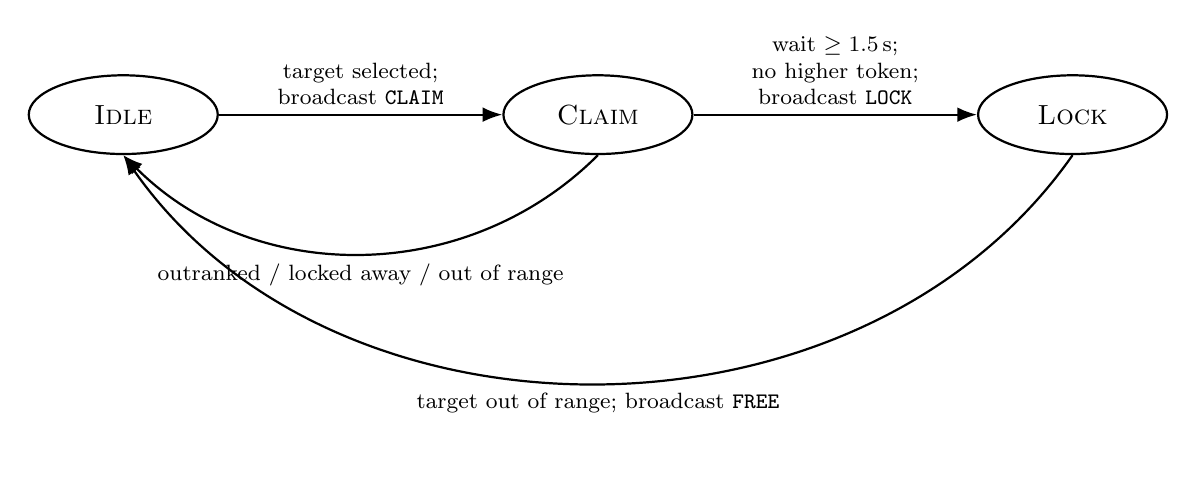
\begin{tikzpicture}[
    node distance=3.5cm and 3.6cm,
    state/.style={ellipse, draw, thick, minimum width=2.4cm, minimum height=1.0cm, align=center},
    arr/.style={-{Latex[length=2.5mm]}, thick},
    lbl/.style={font=\footnotesize, align=center}
]
\node[state] (idle)  {\textsc{Idle}};
\node[state, right=of idle]  (claim) {\textsc{Claim}};
\node[state, right=of claim] (lock)  {\textsc{Lock}};

\draw[arr] (idle)  -- node[lbl, above]{target selected;\\broadcast \texttt{CLAIM}} (claim);
\draw[arr] (claim) -- node[lbl, above]{wait $\geq 1.5$\,s;\\no higher token;\\broadcast \texttt{LOCK}} (lock);

\draw[arr] (claim.south) to[bend left=45]
    node[lbl, below]{outranked / locked away / out of range} (idle.south);
\draw[arr] (lock.south)  to[bend left=55]
    node[lbl, below]{target out of range; broadcast \texttt{FREE}} (idle.south);
\end{tikzpicture}
\caption{State machine executed independently by every UAV. Transitions
are driven by message receipt, the claim-wait timer, and target-range
checks. The diagram omits the self-loop in \textsc{Lock} that
periodically rebroadcasts the \texttt{LOCK} as a heartbeat.}
\label{fig:fsm}
\end{figure}

\subsection{Message Format and Types}
\label{sec:msgs}

All advertisements share a fixed four-field wire format encoded as a
single UTF-8 string:
\[
\langle\,\texttt{msg\_type}\;\;\texttt{uav\_id}\;\;\texttt{target\_id}\;\;\texttt{token}\,\rangle.
\]
The \texttt{msg\_type} field is one of three string literals:

\begin{itemize}
\item \texttt{CLAIM} --- tentative announcement that the sender is
attempting to acquire \texttt{target\_id} with the random tiebreaker
\texttt{token}. Rebroadcast every \texttt{CLAIM\_RETX} seconds while in
\textsc{Claim} so that under loss the claim is heard before the
$1.5$~s wait expires.
\item \texttt{LOCK} --- final announcement that the sender holds
\texttt{target\_id}. Rebroadcast every \texttt{HEARTBEAT\_INTERVAL}
seconds as a liveness signal, and serves as a state-recovery beacon for
peers that started or restarted after the lock was acquired.
\item \texttt{FREE} --- explicit release issued exactly once when a
locked target leaves range, instructing all peers to delete the
sender's entry from their tables immediately.
\end{itemize}

The fixed four-field layout was chosen so that a single
\texttt{recvfrom()} parser handles every message type without a
type-dependent schema. The trade-off is that the \texttt{token} field
is carried even on \texttt{FREE} messages, where it has no semantic
content; this overhead is $\leq 11$~bytes per release and is judged
acceptable.

\subsection{Conflict Resolution}
\label{sec:conflict}

When two or more UAVs \textsc{Claim} the same target concurrently,
exactly one must win and the others must back off. The mechanism is a
random tiebreak token drawn at the start of each claim attempt from
$[1,\,2^{31}-1]$. A UAV in \textsc{Claim} receiving a competing
\textsc{Claim} on its target compares tokens: if the peer's token is
strictly larger, the local UAV abandons its claim, returns to
\textsc{Idle}, and selects a different target on the next tick.

The use of a per-claim random token, rather than the static
\texttt{uav\_id}, satisfies the assignment's explicit requirement that
no node be permanently privileged in tiebreaking. With a $31$-bit token
space, the probability of a token collision between any two UAVs in a
single round is $2^{-31} \approx 4.7\!\times\!10^{-10}$; for the
$N\!=\!8$ swarm evaluated here, the probability that any pair collides
in a single contention is $\binom{8}{2}\!\cdot\!2^{-31} \approx
1.3\!\times\!10^{-8}$. Token collisions are therefore not handled
explicitly --- on the rare event that they occur, both UAVs back off
when neither sees a strictly-larger token, and the next contention
round selects new tokens.

The random number generator on each UAV is seeded at process start with
\[
\texttt{(time\_ns() XOR (my\_id * 2654435761)) \& 0xFFFFFFFF}.
\]
The multiplication by Knuth's $32$-bit hash constant ensures that two UAVs
launched in the same wall-clock nanosecond still produce different
seeds and therefore different first tokens.

\subsection{Timing Parameters}
\label{sec:timing}

The four protocol timers are listed in Table~\ref{tab:timing}. Each
value is justified relative to the others rather than tuned in
isolation.

\begin{table}[h]
\centering
\caption{Protocol timing parameters, with justification.}
\label{tab:timing}
\renewcommand{\arraystretch}{1.25}
\begin{tabular}{@{}l c p{8.5cm}@{}}
\toprule
\textbf{Parameter} & \textbf{Value} & \textbf{Justification} \\
\midrule
\texttt{CLAIM\_WAIT}        & $1.5$~s             & Must exceed the worst-case round trip
                                                     for a tiebreak to arrive before
                                                     \textsc{Claim}$\,\to\,$\textsc{Lock}
                                                     promotion. Bounded above by the
                                                     latency budget of the harness. \\
\texttt{CLAIM\_RETX} (V1)   & $1.0$~s             & One retransmission within the wait
                                                     window; chosen as the baseline. \\
\texttt{CLAIM\_RETX} (V2)   & $0.5$~s             & Three transmissions across the wait
                                                     window. At $20\%$ loss the joint
                                                     loss probability falls from
                                                     $0.20\!\approx\!20\%$ (one transmission)
                                                     and $0.04\!\approx\!4\%$ (V1, two
                                                     transmissions) to
                                                     $0.20^3\!=\!0.008\!\approx\!0.8\%$. \\
\texttt{HEARTBEAT\_INTERVAL}& $1.0$~s             & Cadence at which a \textsc{Lock} is
                                                     rebroadcast. Must be well below
                                                     \texttt{PEER\_TIMEOUT}; chosen as
                                                     $1/4$ of it. \\
\texttt{PEER\_TIMEOUT}      & $4.0$~s             & Number of seconds without a heartbeat
                                                     after which a peer entry is treated
                                                     as crashed. Set to allow up to three
                                                     consecutive heartbeat losses
                                                     ($0.20^3\!\approx\!0.8\%$ false-eviction
                                                     probability) before age-out. \\
\bottomrule
\end{tabular}
\end{table}

The two evaluated variants of the protocol differ only in
\texttt{CLAIM\_RETX}; all other timers are held constant.

\subsection{Fault Tolerance}
\label{sec:fault}

Two failure modes are addressed by the protocol:

\textit{UAV crash.} A UAV that has acquired a \textsc{Lock} and then
crashes without sending \texttt{FREE} would, in a naive design,
permanently remove its target from the assignable set. Each peer
therefore time-stamps the most recent advertisement received from every
UAV and ages out entries whose timestamp exceeds \texttt{PEER\_TIMEOUT}.
Once an entry is evicted, the target it held becomes assignable again
on the next \textsc{Idle} tick. No coordination is required for this
recovery; each peer prunes its own table independently.

\textit{Target out of range.} A locked UAV that loses range on its
target broadcasts \texttt{FREE} and returns to \textsc{Idle}. The
explicit \texttt{FREE} causes peers to release the entry immediately
rather than waiting up to $4$~s for peer-timeout, which is important
when a different UAV is in range of the released target and would
otherwise spend the timeout window unable to claim it.

% =====================================================================
\section{Results}
% =====================================================================

The protocol was evaluated on a CORE 7.1.0 emulation with $8$~UAVs and
$8$~targets sharing wlan21. Three configurations were measured: an
\textit{ideal} channel (no induced loss or delay), a \textit{realistic}
channel with $20\%$ loss and $200$~ms delay running protocol variant
V1 (\texttt{CLAIM\_RETX}\,$=\,1.0$~s), and the same realistic channel
running variant V2 (\texttt{CLAIM\_RETX}\,$=\,0.5$~s). Each
configuration was evaluated across the harness's eight test cases
covering sequential arrival (1a, 1b), partial coverage (2a, 2b),
simultaneous arrival (3a, 3b), and crashed-UAV scenarios (4, 5).

\subsection{Correctness}
\label{sec:correct}

Per-test outcomes are summarised in Table~\ref{tab:correct}. The
aggregate pass counts are $8/8$ ideal, $4/8$ realistic-V1, and $5/8$
realistic-V2.

\begin{table}[h]
\centering
\caption{Per-test correctness across the three configurations.
\checkmark\ denotes a passing test (all UAVs locked to distinct
targets); \ding{55}\ denotes a failure (at least one duplicate
assignment).}
\label{tab:correct}
\renewcommand{\arraystretch}{1.2}
\begin{tabular}{@{}l c c c@{}}
\toprule
\textbf{Test} & \textbf{Ideal} & \textbf{Realistic V1} & \textbf{Realistic V2} \\
\midrule
1a (sequential, in order)         & \checkmark & \ding{55}  & \checkmark \\
1b (sequential, out of order)     & \checkmark & \ding{55}  & \ding{55}  \\
2a (partial, in order)            & \checkmark & \checkmark & \checkmark \\
2b (partial, out of order)        & \checkmark & \checkmark & \checkmark \\
3a (simultaneous, in order)       & \checkmark & \checkmark & \ding{55}  \\
3b (simultaneous, out of order)   & \checkmark & \ding{55}  & \ding{55}  \\
4  (1 crashed UAV)                & \checkmark & \checkmark & \checkmark \\
5  (2 crashed UAVs)               & \checkmark & \ding{55}  & \checkmark \\
\midrule
\textbf{Total passes}             & \textbf{8/8} & \textbf{4/8} & \textbf{5/8} \\
\bottomrule
\end{tabular}
\end{table}

The ideal column shows that the protocol is correct in the absence of
loss and delay, confirming that the state machine, message format, and
tiebreaking logic implement the assignment specification. The
realistic columns are interpreted in Section~\ref{sec:disc}.

\subsection{Latency}
\label{sec:lat}

End-to-end latency was measured by the harness as the elapsed time from
the first target movement command to the moment all surviving UAVs had
recorded their final assignments. Per-test values are listed in
Table~\ref{tab:lat}. Means across all eight tests are $8.99$~s (ideal),
$10.42$~s (V1), and $10.72$~s (V2).

\begin{table}[h]
\centering
\caption{Per-test latency in seconds.}
\label{tab:lat}
\renewcommand{\arraystretch}{1.2}
\begin{tabular}{@{}l c c c@{}}
\toprule
\textbf{Test} & \textbf{Ideal} & \textbf{Realistic V1} & \textbf{Realistic V2} \\
\midrule
1a   & 16.17 & 16.15 & 16.14 \\
1b   & 16.21 & 16.17 & 16.15 \\
2a   & 12.22 & 13.02 & 12.71 \\
2b   & 12.16 & 12.13 & 14.23 \\
3a   &  4.51 &  7.64 &  6.85 \\
3b   &  4.27 &  7.01 &  6.92 \\
4    &  3.21 &  4.87 &  6.82 \\
5    &  3.17 &  6.39 &  5.90 \\
\midrule
\textbf{Mean} & \textbf{8.99} & \textbf{10.42} & \textbf{10.72} \\
\bottomrule
\end{tabular}
\end{table}

Two observations follow directly from the data. First, tests 1a, 1b,
2a, and 2b sit very close to a $16$~s ceiling on every configuration.
This ceiling is imposed by the harness, not the protocol: it issues
target movements at a fixed $2$~s inter-arrival interval, so the final
target in an eight-target test cannot become assignable before
$\sim\!14$~s. Second, the simultaneous-arrival tests (3a, 3b) and the
crash tests (4, 5) show a clean increase from ideal to realistic
($\sim\!4$~s$\,\to\,\sim\!7$~s and $\sim\!3$~s$\,\to\,\sim\!6$~s
respectively). This residual is the actual cost of the channel
impairments: under loss, more rounds of \textsc{Claim} contention are
required before the swarm converges.

The mean latency increases by $1.43$~s from ideal to V1 and by a
further $0.30$~s from V1 to V2. The latter increment is small enough
to be within the noise of the eight-test sample, indicating that the
faster claim retransmission of V2 does not materially raise mean
completion time.

\subsection{Throughput}
\label{sec:thru}

Per-node throughput traces for the three configurations are shown in
Figs.~\ref{fig:thru-ideal}--\ref{fig:thru-v2}. All three plots share
the same $y$-axis range ($0$--$10$~kbps) for direct visual comparison.

\begin{figure}[h]
\centering
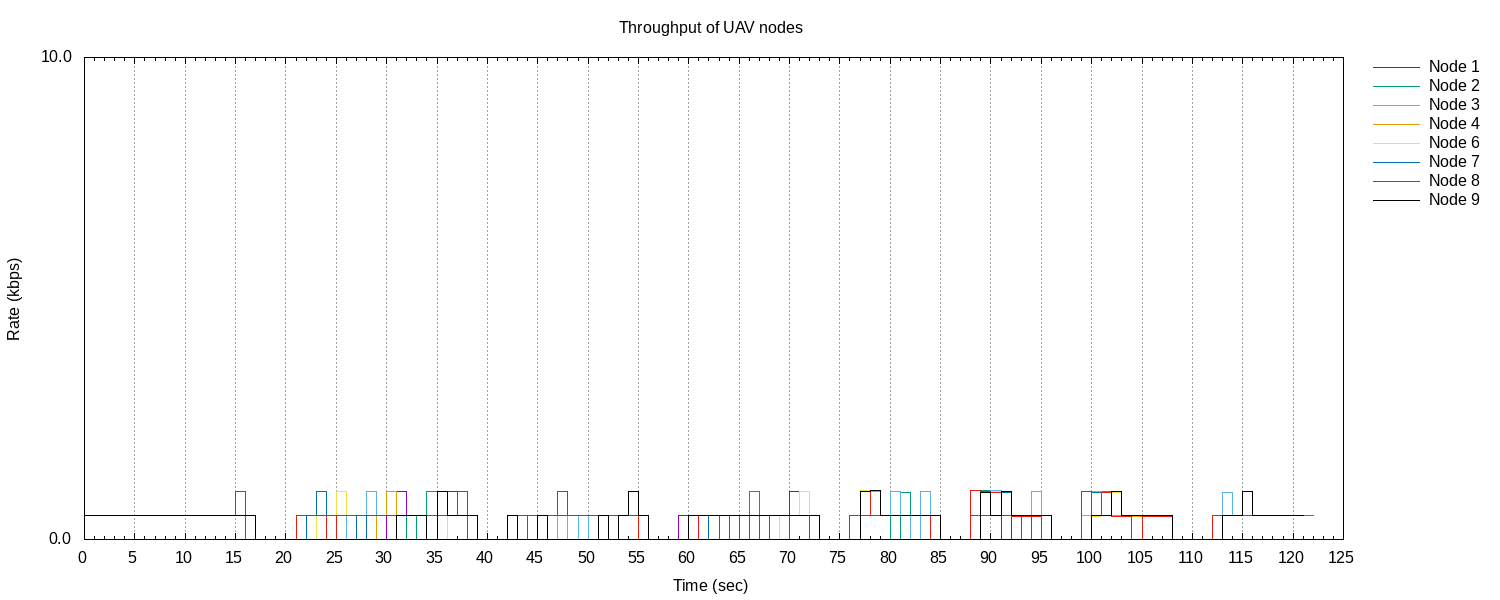
\includegraphics[width=\linewidth]{figures/uavs_throughput_plot_ideal.png}
\caption{Per-UAV throughput, ideal channel. Activity is sparse and
concentrated in short bursts at each test event.}
\label{fig:thru-ideal}
\end{figure}

\begin{figure}[h]
\centering
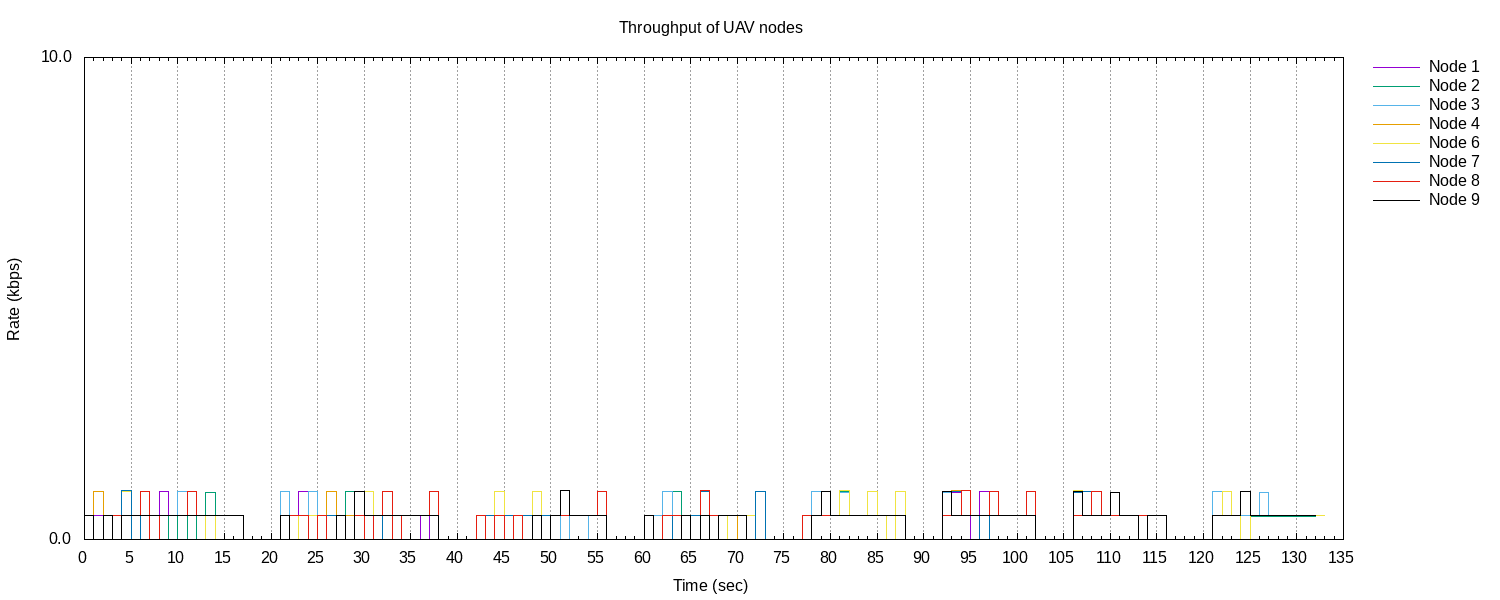
\includegraphics[width=\linewidth]{figures/uavs_throughput_plot_realistic_V1.png}
\caption{Per-UAV throughput, realistic channel ($20\%$ loss,
$200$~ms delay), variant V1 (\texttt{CLAIM\_RETX}\,$=\,1.0$~s).}
\label{fig:thru-v1}
\end{figure}

\begin{figure}[h!]
\centering
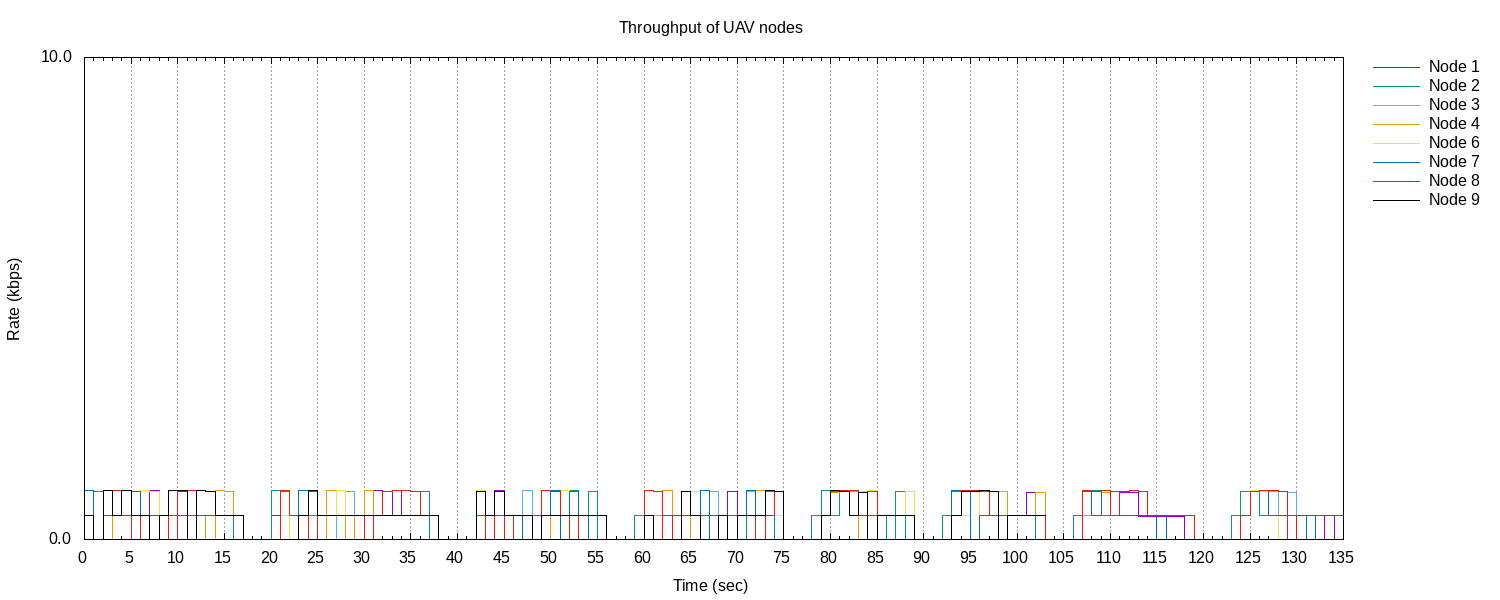
\includegraphics[width=\linewidth]{figures/uavs_throughput_plot_realistic_V2.png}
\caption{Per-UAV throughput, realistic channel ($20\%$ loss,
$200$~ms delay), variant V2 (\texttt{CLAIM\_RETX}\,$=\,0.5$~s).
The trace is visibly denser than V1 due to the doubled
claim-retransmission rate, but the per-node sustained rate remains
below $\sim\!0.5$~kbps.}
\label{fig:thru-v2}
\end{figure}

The sustained per-node rate stays below $\sim\!0.5$~kbps in all three
plots, dominated by the $1$~Hz \texttt{LOCK} heartbeat once the swarm
has converged. With each advertisement carrying $\leq\!20$~bytes
including UDP/IP headers, $1$~Hz heartbeats correspond to
$\sim\!0.16$~kbps per node, consistent with the observed traces.
The visible difference between V1 (Fig.~\ref{fig:thru-v1}) and V2
(Fig.~\ref{fig:thru-v2}) is not in peak rate but in trace
\textit{density}: V2 shows more frequent transmission events during
contention windows, which is the mechanism by which V2 reduces joint
loss probability (Section~\ref{sec:disc}). The aggregate offered load
is therefore slightly higher under V2, but remains negligible relative
to the channel capacity.

% =====================================================================
\section{Discussion}
\label{sec:disc}
% =====================================================================

This section interprets the correctness results in
Table~\ref{tab:correct}, identifies the mechanism that drives the
realistic-channel failures, compares the two protocol variants, and
states the limitations of the design.

\subsection{Tests 2a, 2b, and 4}

Tests 2a, 2b, and 4 pass on every configuration. In these tests the
number of in-range targets is, at any given moment, comparable to or
smaller than the number of competing UAVs, and the targets become
assignable in a staggered pattern that lets each UAV's
\textit{potential-target list} differ from its neighbours'. The
consequence is that two UAVs rarely select the same candidate target
in the same tick, contention is localised to small subsets of the
swarm, and the few \textsc{Claim} collisions that do occur are
resolved within one \texttt{CLAIM\_WAIT} window. Loss and delay still
affect these tests --- their latency rises from $\sim\!3$~s to
$\sim\!5$--$7$~s --- but correctness is preserved because a single
unrecovered tiebreak still has alternative targets to fall back on.

\subsection{Tests 1a, 1b, 3a, and 3b}

Tests 1a, 1b, 3a, and 3b expose the protocol's central weakness. In the
sequential tests (1a, 1b) targets arrive one at a time, so all
$8$~UAVs have nearly identical potential-target lists and contend for
the same single new target on every $2$~s arrival. In the simultaneous
tests (3a, 3b) all eight targets become assignable at once, producing
maximum contention in a single tick.

Under realistic conditions ($20\%$ loss, $200$~ms one-way delay), the
mechanism that fails is the tiebreak path itself. For a UAV $A$ to
correctly defer to a higher-token claim from UAV $B$, $B$'s
\texttt{CLAIM} message must (i) traverse the channel without being
dropped and (ii) arrive before $A$'s \texttt{CLAIM\_WAIT} timer
expires. The probability that $B$'s claim is lost on every
retransmission within the $1.5$~s wait window is $p^{k}$, where
$p\!=\!0.20$ is the per-packet loss probability and $k$ is the number
of transmissions $B$ issues during the window. With V1's
\texttt{CLAIM\_RETX}\,$=\,1.0$~s, $B$ transmits twice within the
window (initial plus one retransmission), giving a joint loss of
$0.20^{2}\!=\!4\%$ \textit{per contender pair}. Across an eight-way
contention there are $\binom{8}{2}\!=\!28$ pairs, and the probability
that at least one pair fails to hear each other is
$1\!-\!(1\!-\!0.04)^{28} \approx 68\%$. Once a tiebreak is missed, both
UAVs promote \textsc{Claim} to \textsc{Lock} on the same target, and
the lock-once-acquired constraint prevents either from releasing it
voluntarily --- the duplicate persists for the remainder of the test.
This is the failure mode visible in 1a, 1b, and 3b under V1.

\subsection{V1 versus V2: Halving the Joint-Loss Probability}

V2 raises the number of claim transmissions per wait window from $2$
to $3$ by halving \texttt{CLAIM\_RETX}. The per-pair joint loss falls
from $0.20^{2}\!=\!4\%$ to $0.20^{3}\!=\!0.8\%$, and the per-test
probability of at least one missed tiebreak across $28$ pairs falls
from $\sim\!68\%$ to $\sim\!20\%$. The empirical pass rate moves in the
predicted direction: $4/8$ under V1, $5/8$ under V2.

V2 recovers test~1a (the in-order sequential case) and test~5 (two
crashed UAVs) but loses test~3a (in-order simultaneous arrival), which
V1 had passed. With only one trial per case, this pattern cannot be
distinguished from sampling noise on a $28$-pair tiebreak process whose
per-test failure probability is in the $20$--$70\%$ range. The
aggregate improvement of $+1$ test is consistent with the predicted
reduction in joint loss, but the per-case shuffle should be
interpreted as variance, not as evidence that V2 is worse on simultaneous
arrival.

Mean latency is essentially unchanged between V1 and V2 ($10.42$~s vs.\
$10.72$~s, a $3\%$ difference). The faster retransmission rate
therefore buys correctness improvement at no measurable latency cost.

\subsection{Fault Tolerance under Loss}

Tests~4 and 5 evaluate behaviour when one or two UAVs are crashed
before the test begins. Under ideal conditions both pass trivially.
Under realistic conditions, test~4 passes on both variants and test~5
passes only on V2. The mechanism is the
\texttt{PEER\_TIMEOUT}-based eviction described in
Section~\ref{sec:fault}: once a crashed UAV's heartbeats stop arriving,
the remaining peers prune its entry from their tables within $4$~s,
after which the surviving swarm has \textit{fewer} contenders for the
same target set. In other words, crashing UAVs reduces contention,
which makes the assignment problem strictly easier than the
no-crash baseline, not harder. The failure of test~5 under V1 is
therefore not a fault-tolerance failure but the same wait-window-bound
failure that affects 1a, 1b, and 3b: the surviving six UAVs still
contend over a single new target at each arrival, and one tiebreak in
$28$ goes unheard.

\subsection{Limitations}
\label{sec:lim}

The protocol and its evaluation have several limitations that should
be stated explicitly.

\textit{Single-phase commit.} The promotion rule from \textsc{Claim}
to \textsc{Lock} requires only that no higher-token contender be heard
within \texttt{CLAIM\_WAIT}. A UAV that does not hear a contender's
claim --- whether because the claim was dropped or because it arrived
after the wait expired --- promotes regardless. The protocol has no
acknowledgement step that would let a claimant verify, before
promoting, that all peers have observed its claim. This is the
fundamental cause of the realistic-channel failures.

\textit{Static wait window.} \texttt{CLAIM\_WAIT} is a fixed $1.5$~s
constant. It is not adapted to the measured RTT or loss rate of the
channel. On a channel where the actual RTT is much smaller than
$1.5$~s, the protocol pays unnecessary latency; on a channel where
loss bursts exceed three consecutive packets per UAV pair, the wait
window cannot accommodate them regardless of \texttt{CLAIM\_RETX}.

\textit{No exponential backoff on retransmission.}
\texttt{CLAIM\_RETX} is a fixed period. Under contention bursts where
many UAVs claim simultaneously, all of them retransmit on the same
cadence, producing correlated transmission times that increase the
effective collision probability on the shared medium.

\textit{Lock-once-never-released constraint.} The assignment requires
that once a UAV \textsc{Lock}s a target, that lock is not released
unless the target leaves range. This eliminates by construction any
recovery mechanism for the duplicate-lock failure mode in
Section~\ref{sec:disc}. Once two UAVs have promoted to \textsc{Lock}
on the same target, the protocol cannot heal the assignment.

% \textit{Single trial per case.} Each cell of Table~\ref{tab:correct}
% reflects one test execution. The per-case pass/fail pattern is
% therefore subject to substantial variance and should not be
% interpreted as a stable estimator of any individual case's success
% probability. The aggregate counts ($8/8$, $4/8$, $5/8$) are more
% robust because they integrate over eight independent tests, but they
% remain a sample of size eight.

% \textit{Scope.} The evaluation covers an $8$-UAV, $8$-target swarm on
% a single shared wireless medium, with channel impairment limited to
% i.i.d.\ packet loss and constant one-way delay. Variable swarm size,
% mobility-induced topology changes, bursty loss, and asymmetric delay
% are out of scope.

\end{document}
